\section{NETWORK SERVER CONFIGURATION}

In this case, the Network Server is an instance of \texttt{ResIoT}\cite{ResIOTLoRaWANNetwork}. This instance needs to be configured for each node created.

\subsection{Node configuration}

For this case, the node follows the next configuration and definitions:
\begin{itemize}
    \item \textbf{Type of activation}: In this project, the node uses \acrfullr{otaa}, which gives the possibility of changing the network on startup. 
    This method needs some configuration in the node in the form of some identifiers and an \texttt{APP\_KEY}.The configuration for the device is done in 
    the main module and can be seen in \autoref{fig:nodeconfig}.
    \begin{figure}[H]
        \centering
        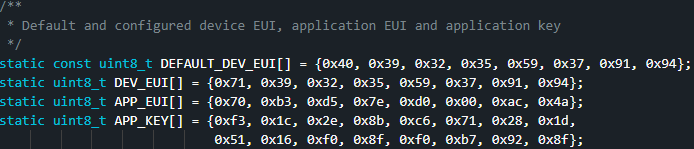
\includegraphics[width=0.85\textwidth]{images/6/Node_config.png}
        \caption{Configuration for the \texttt{OTAA} in the node}
        \label{fig:nodeconfig}
    \end{figure}
    \begin{itemize}
        \item \texttt{DEV\_EUI}: The unique identifier specified by the teachers, in this project, the first byte is $0x71$.
        \item \texttt{APP\_EUI}: The unique identifier for the end application in the network server.
        \item \texttt{APP\_KEY}: This key is used to generate the two keys for the MAC layer and the payload.
    \end{itemize}
    \item \textbf{Type of device}: the node works in class A of \acrshort{lorawan}. It will open 2 specific RX windows after a TX.
\end{itemize}

\subsection{Node definition in the network server}

In the network server, a node was defined with the next characteristics:
\begin{itemize}
    \item \textbf{Name}: \texttt{NODE\_SN\_GROUP\_A}.
    \item \textbf{Node AUTH}: \texttt{LoRaWAN OTAA Class A}.
    \item \textbf{Device EUI}: The same defined in the node configuration in \autoref{fig:nodeconfig}.
    \item \textbf{Application}: The app that shares the same \texttt{APP\_EUI} as in the \autoref{fig:nodeconfig}. In this case, \\ \texttt{RRSS2024\_AppEUI}, that has the configuration of \autoref{fig:appconfig}.
    \begin{figure}[H]
        \centering
        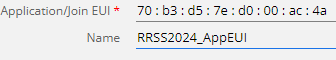
\includegraphics[width=0.6\textwidth]{images/6/AppName.png}
        \caption{App configuration in the network server}
        \label{fig:appconfig}
    \end{figure}
    \item \textbf{APP\_KEY}: The same defined in the node configuration in \autoref{fig:nodeconfig}.
    \item \textbf{LoRaWAN Network Server}: This field points to the server ``eu72.resiot.io\:7677'', configured as a \acrshort{lorawan} Europe server (\texttt{868 MHz}) for Class A+C nodes.
    \item \textbf{Advanced LoRaWAN configuration}: the most important one is that it has \acrfullr{adr}. The reception windows offset are also by default.
    \item \textbf{Node Fields}:
\end{itemize}
\clearpage
\subsection{LUA Scripting}
\clearpage
\subsection{Dashboard design}
\clearpage